% !TEX TS-program = pdflatex
% !TEX encoding = UTF-8 Unicode
\documentclass[12pt]{article} 

\usepackage[utf8]{inputenc} 
\usepackage{geometry} 
\geometry{a4paper} 
\geometry{margin=0.25in} 
\geometry{portrait} 

\usepackage{tikz} 

\usepackage{amsmath} 
\usepackage{physics} 
\usetikzlibrary{shapes.geometric}

\title{fbds}

\author{vijayabhaskar badireddi} 

\begin{document} 

\section*{Free body diagrams}
%\subsection*{projectile}

\begin{center}
\begin{tikzpicture}

\datavisualization [school book axes, visualize as smooth line]

data [format=function] {
var x : interval [-1.5:1.5] samples 10 ;
func y = \value x * \value x;
} ;

\end{tikzpicture}
\end{center}

%% !TEX root = fbds.tex

\subsection*{ramp}

\begin{center}
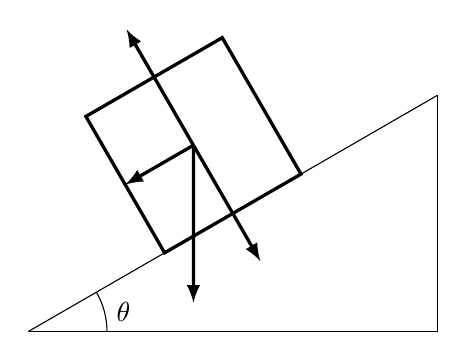
\begin{tikzpicture}
\draw (0,0) -- (30:6) ;
\draw (30:6) -- ++(0,-3) -- (0,0) ;
\draw (1,0) arc [start angle = 0, end angle =30, radius =1] ;
\draw node at (1,0) [anchor=south west] {$\theta$} ;
\draw [very thick,rotate=30] (0:2) rectangle ++(2,2) ; 
\draw [very thick,rotate=30,-{latex}] (0:3) ++(0,1) -- ++(-1,0) ; 
\draw [very thick,rotate=30,-{latex}] (0:3) ++(0,1) -- ++(0,-1.7) ; 
\draw [very thick,rotate=30,-{latex}] (0:3) ++(0,1) -- ++(-120:2) ;
\draw [very thick,rotate=30,-{latex}] (0:3) ++(0,1) -- ++(0,1.7) ;
\end{tikzpicture}
\end{center}
%\subsection*{pulley4}

\begin{center}
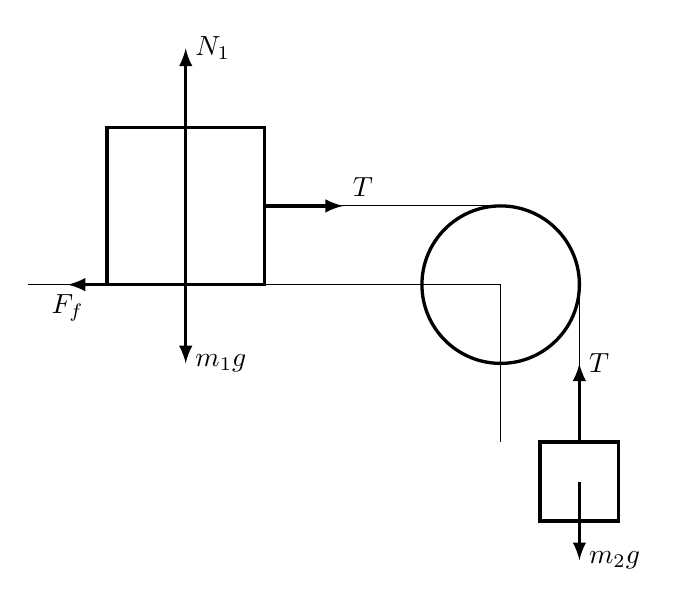
\begin{tikzpicture}

\draw (-6,0) -- (0,0) ;
\draw [very thick] (0,0) circle [radius=1] ;
\draw (1,0) -- (1,-2) ;
\draw (0,0) -- (0,-2) ;
\draw [very thick] (0.5,-3) rectangle (1.5,-2) ;
\draw (-3,1) -- (0,1) ;
\draw [very thick] (-5,0) rectangle (-3,2) ;
\draw [very thick, -{latex}] (-3,1) -- (-2,1) ;
\draw node at (-4,-1) [anchor=west] {$m_1g$} ;  
\draw [very thick, -{latex}] (1,-2.5) -- (1,-3.5) ;
\draw [very thick, -{latex}] (1,-2) -- (1,-1) ;
\draw node at (1,-3.5) [anchor=west] {$m_2g$} ;
\draw node at (1,-1) [anchor=west] {$T$} ;
\draw node at (-2,1) [anchor=south west] {$T$} ;
\draw [very thick, -{latex}] (-4,1) -- (-4,-1) ;
\draw [very thick, -{latex}] (-4,1) -- (-4,3) ;
\draw node at (-4,3) [anchor=west] {$N_1$} ;
\draw node at (-5.5,0) [anchor=north] {$F_f$} ;
\draw [very thick, -{latex}] (-4,0) -- (-5.5,0) ;
\end{tikzpicture}
\end{center}

\subsection*{inclined plane}

\begin{center}
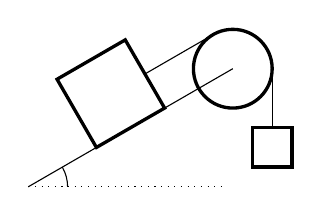
\begin{tikzpicture}[scale=0.5]

\draw [dotted] (0,0) -- (5,0) ;
\draw (0,0) -- ++(30:6) ;
\draw (1,0) arc [start angle=0,end angle=30,radius=1] ;
\draw [very thick] (30:6) circle [radius=1];
\draw (30:6) ++(0:1) -- ++(-90:1.5) ;
\draw [very thick] (30:6) ++(0:1) ++(-90:1.5) ++(-0.5,-1) rectangle ++(1,1) ;
\draw [very thick,rotate=30] (0:2) rectangle ++(2,2);
\draw (30:4) ++(120:1) -- ++(30:2) ; 

\end{tikzpicture}
\end{center}
%\subsection*{hanging string}

\begin{center}
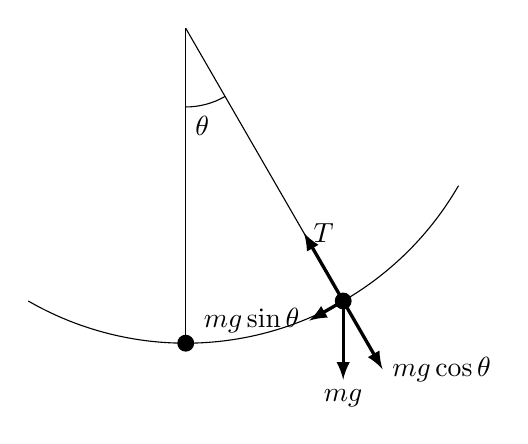
\begin{tikzpicture}

\draw (0,-4) arc [start angle=-90, end angle= -30, radius = 4] ;
\draw (0,-4) arc [start angle=-90, end angle= -120, radius = 4] ;
\draw (0,0) -- (0,-4) ;
\draw [fill] (0,-4) circle [radius=0.1] ; 
\draw [fill] (-60:4) circle [radius=0.1] ;
\draw (0,0) -- (-60:4) ;
\draw (0,-1) arc [start angle =-90, end angle=-60,radius=1] ;
\draw (0,-1) node [anchor=north west] {$\theta$} ;
\draw [very thick,-{latex}] (-60:4) -- ++(0,-1) ;
\draw (-60:4) ++(0,-1) node [anchor=north] {$mg$} ;
\draw [very thick,-{latex}] (-60:4) -- ++(-150:0.5) ;
\draw (-60:4) ++(-150:0.5) node [anchor=east] {$mg\sin\theta$} ;
\draw [very thick,-{latex}] (-60:4) -- ++(-60:1) ;
\draw (-60:4) ++(-60:1) node [anchor=west] {$mg\cos\theta$} ;
\draw [very thick,-{latex}] (-60:4) -- ++(120:1) ;
\draw (-60:4) ++(120:1) node [anchor=west] {$T$} ;

\end{tikzpicture}
\end{center}
%\subsection*{pulley system 3}

\begin{center}
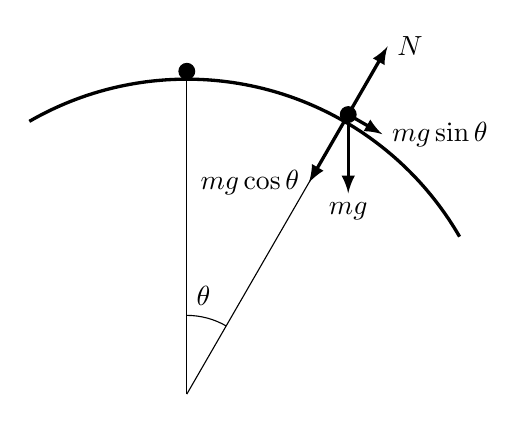
\begin{tikzpicture}[scale=1]

\draw [very thick] (0,4) arc [start angle=90, end angle= 30, radius = 4] ;
\draw [very thick] (0,4) arc [start angle=90, end angle= 120, radius = 4] ;
\draw (0,0) -- (0,4) ;
\draw [fill] (0,4.1) circle [radius=0.1] ; 
\draw [fill] (60:4.1) circle [radius=0.1] ;
\draw (0,0) -- (60:4) ;
\draw (0,1) arc [start angle =90, end angle=60,radius=1] ;
\draw (0,1) node [anchor=south west] {$\theta$} ;
\draw [very thick,-{latex}] (60:4.1) -- ++(0,-1) ;
\draw (60:4.1) ++(0,-1) node [anchor=north] {$mg$} ;
\draw [very thick,-{latex}] (60:4.1) -- ++(-120:1) ;
\draw (60:4.1) ++(-120:1) node [anchor=east] {$mg\cos\theta$} ;
\draw [very thick,-{latex}] (60:4.1) -- ++(60:1) ;
\draw (60:4.1) ++(-30:0.5) node [anchor=west] {$mg\sin\theta$} ;
\draw [very thick,-{latex}] (60:4.1) -- ++(-30:0.5) ;
\draw (60:4.1) ++(60:1) node [anchor=west] {$N$} ;

\end{tikzpicture}
\end{center}

%\subsection*{pulley system 2}

\begin{center}
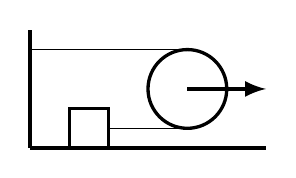
\begin{tikzpicture}[scale=0.5]

\draw [ultra thick] (0,0) -- (6,0) ;
\draw [ultra thick] (0,0) -- (0,3) ;
\draw [very thick] (4,1.5) circle [radius=1] ;
\draw (0,2.5) -- (4,2.5) ;
\draw (2,0.5) -- (4,0.5) ;
\draw [very thick] (1,0) rectangle ++(1,1);
\draw [ultra thick,-{latex}] (4,1.5) -- (6,1.5) ;
\end{tikzpicture}
\end{center}
%% !TeX root = figures.tex

\subsection*{pulley system 1}

\begin{center}
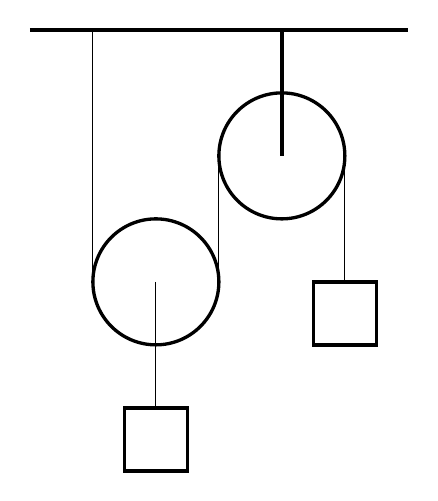
\begin{tikzpicture}[scale=0.8]

\draw [ultra thick] (0,0) -- (6,0) ;
\draw [very thick] (2,-4) circle [radius=1] ;
\draw [very thick] (4,-2) circle [radius=1] ;
\draw (1,0) -- (1,-4) (3,-4) -- (3,-2) (5,-2) -- (5,-4) ;
\draw (2,-4) -- (2,-6) ; 
\draw [very thick] (4,0) -- (4,-2) ;
\draw [very thick] (2,-6) ++(-0.5,-1) rectangle ++(1,1) ;
\draw [very thick] (5,-4) ++(-0.5,-1) rectangle ++(1,1) ;
\end{tikzpicture}
\end{center}
%\subsection*{pendulum}

\begin{center}
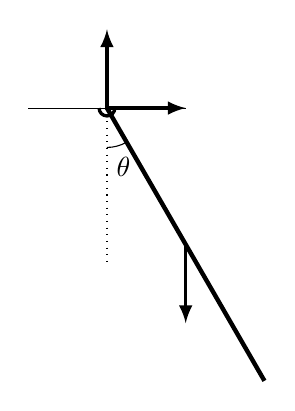
\begin{tikzpicture}

\draw (-1,0) -- (1,0) ;
\draw [very thick] (-0.1,0) arc  [start angle=-180,end angle=0,radius=0.1] ;
\draw [dotted] (0,0) -- (0,-2) ; 
\draw [ultra thick] (0,0) -- (-60:4) ;
\draw (0,-0.5) arc  [start angle=-90,end angle=-60,radius=0.5] ;
\draw (0,-0.5) node [anchor=north west] {$\theta$} ;
\draw [very thick,-{latex}] (-60:2) -- ++(0,-1) ;
\draw [very thick,-{latex}] (0,0) -- ++(0,1) ;
\draw [very thick,-{latex}] (0,0) -- ++(1,0) ; 

\end{tikzpicture}
\end{center}
%\subsection*{ladder1}

\begin{center}
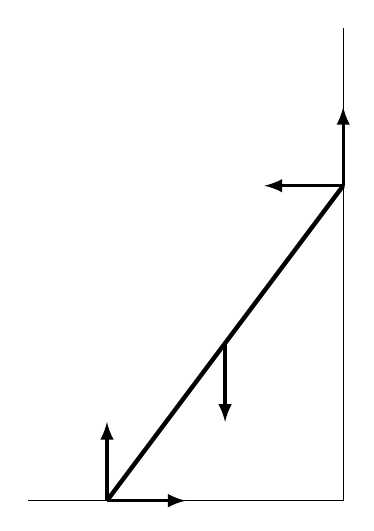
\begin{tikzpicture}

\draw (-4,0) -- (0,0) ;
\draw (0,0) -- (0,6) ;
\draw [ultra thick] (-3,0) -- (0,4) ;
\draw [very thick,-{latex}] (0,4) -- ++(0,1) ;
\draw [very thick,-{latex}] (0,4) -- ++(-1,0) ;
\draw [very thick,-{latex}] (-3,0) -- ++(0,1) ;
\draw [very thick,-{latex}] (-3,0) -- ++(1,0) ;
\draw [very thick,-{latex}] (-1.5,2) -- ++(0,-1) ; 

\end{tikzpicture}
\end{center}

%\subsection*{ladder2}

\begin{center}
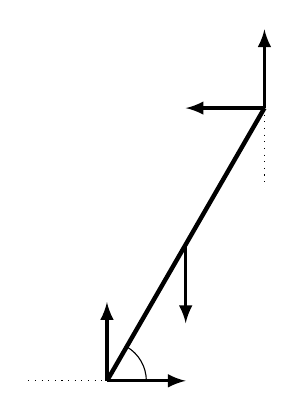
\begin{tikzpicture}
\draw [dotted] (-1,0) -- (1,0) ;
\draw [dotted] (60:4) -- ++(0,1) ;
\draw [dotted] (60:4) -- ++(0,-1) ;
\draw (0.5,0) arc [start angle = 0, end angle = 60, radius=0.5] ;
\draw [ultra thick] (0,0) -- ++(60:4) ;
\draw [very thick,-{latex}] (60:4) -- ++(0,1) ;
\draw [very thick,-{latex}] (60:4) -- ++(-1,0) ;
\draw [very thick,-{latex}] (0,0) -- ++(0,1) ;
\draw [very thick,-{latex}] (0,0) -- ++(1,0) ;
\draw [very thick,-{latex}] (60:2) -- ++(0,-1) ; 

\end{tikzpicture}
\end{center}

\end{document}
